\chapter{Experimenten}
\label{ch:experimenten}

De implementatie van de verschillende objectdetectiemodellen vormt de belangrijkste voorbereidende stap in het ontwikkelen van de ``proof of concept'' voor dit onderzoek. In deze fase wordt de theorie over de verschillende modelarchitecturen (zie \ref{ch:stand-van-zaken}) vertaald naar praktische, werkende systemen. Dit omvat het selecteren van een geschikte detectiemethode per categorie -- zowel supervised, semi-supervised en self-supervised -- en het configureren en connecteren van de verschillende componenten. Daarnaast wordt er aandacht besteed aan de optimalisatie-instellingen -- zoals learning rate schedules -- die van grote invloed (kunnen) zijn op de prestaties. Ook zal het gekozen deep learning-framework worden besproken en toegelicht. In dit hoofdstuk wordt beschreven hoe de gekozen modellen zijn geïmplementeerd, welke architecturale keuzes zijn gemaakt, en hoe deze implementatie is afgestemd op de specifieke kenmerken van de dataset en de uiteindelijke toepassing. Zo wordt de basis gelegd voor het daaropvolgende trainingsproces.

% Experimentele setup
\section{Experimentele setup}

\subsection{Deep learning frameworks en tools}

Vandaag de dag bestaan er verschillende deep learning frameworks die de ontwikkeling en implementatie van neurale netwerken sterk vergemakkelijken. Enkele van de meest gebruikte zijn TensorFlow, PyTorch, JAX en Keras. TensorFlow en PyTorch zijn de twee dominante deep learning frameworks in het veld van artificiële intelligentie. Keras is een speciale uitzondering: het is namelijk een bibliotheek die compatibiliteit biedt tussen deze verschillende frameworks.

\subsubsection{TensorFlow}

TensorFlow (geïntroduceerd door Google in 2015) werd ontworpen met het oog op grootschalige productieomgevingen. Het framework biedt uitgebreide ondersteuning voor het deployen van modellen op verschillende platformen, zoals mobiele apparaten en webapplicaties, en beschikt over geavanceerde tools zoals TensorBoard voor visualisatie en TensorFlow Serving voor schaalbare modelinzet. TensorFlow’s aanpak met statische computationele grafen (in vroege versies) maakte het echter aanvankelijk minder intuïtief voor onderzoek en experimentatie, hoewel TensorFlow 2.x dit deels heeft verbeterd door de introductie van \emph{eager execution}. TensorFlow biedt ook veruit de beste integratie met \glspl{tpu}. \autocite{Pang_2019}

\subsubsection{PyTorch}

PyTorch (ontwikkeld door \gls{fair} en uitgebracht in 2016) heeft daarentegen vanaf het begin sterk ingezet op gebruiksvriendelijkheid en flexibiliteit. PyTorch maakt gebruik van dynamische computationele grafen, wat betekent dat het netwerk direct kan worden aangepast tijdens de uitvoering. Dit maakt het debuggen eenvoudiger en laat onderzoekers sneller experimenteren met nieuwe architecturen en technieken. Bovendien sluit de programmeerstijl van PyTorch dichter aan bij standaard Python, wat de leercurve verlaagt en de ontwikkelsnelheid verhoogt. In de onderzoekswereld heeft PyTorch hierdoor snel populariteit gewonnen, en veel state-of-the-art modellen en papers publiceren tegenwoordig hun codebase standaard in PyTorch. \autocite{Imambi_2021} \\

Voor dit project is uiteindelijk gekozen voor PyTorch vanwege de flexibiliteit en transparantie die het biedt tijdens het ontwikkelen en experimenteren met objectdetectiemodellen. PyTorch biedt namelijk uitstekende integraties met moderne detectiebibliotheken zoals TorchVision, wat de implementatie en evaluatie van complexe modellen versnelt. Daarnaast is het makkelijk om gepretrainde detectiemodellen te importeren, waardoor in dit onderzoek gefocust kan worden op de nieuwe ontwikkelingen zonder de focus te moeten verschuiven naar complexe backbones. Ook de installatie, configuratie en setup van PyTorch zijn veel eenvoudiger dan bij TensorFlow. Deze eigenschappen maken PyTorch tot de meest geschikte keuze om de doelstellingen van dit onderzoek efficiënt en effectief te realiseren.

\subsection{Hardware en compute resources}

Het trainen van deze objectdetectiemodellen is een intensief proces dat zowel op het vlak van data als computationele resources aanzienlijke vereisten stelt. Zoals uitgelegd in \ref{subsec:definitie-en-gebruik-op-sonarafbeeldingen} combineert objectdetectie classificatie en lokalisatie: het model moet niet alleen herkennen wat er in een afbeelding aanwezig is, maar ook waar het zich bevindt via het voorspellen van \glspl{bounding_box}. Tijdens het trainingsproces worden geannoteerde datasets gebruikt waarbij objecten met klasse-labels en coördinaten zijn aangeduid, zoals in \gls{coco} of Pascal \gls{voc}. Het model leert via een samengestelde \gls{loss_functie}, die typisch zowel classificatiefouten als fouten in de \glspl{bounding_box} omvat. Door middel van \gls{backpropagation} worden de gewichten van het neurale netwerk aangepast om deze gecombineerde \gls{loss_functie} te minimaliseren. Omdat objectdetectie vaak gebaseerd is op diepe \glspl{cnn}, vereist het trainingsproces krachtige hardware. \\

\subsubsection{CPU / GPU / TPU}

Omwille van deze vereisten, worden neurale netwerken vrijwel nooit getraind op \glspl{cpu}. Een \gls{cpu} is namelijk zeer goed in het uitvoeren van \emph{general-purpose} taken (besturingssysteem draaien, tekstverwerking, spreadsheets \dots) op een sequentiële manier. Om hiervoor geoptimaliseerd te zijn, bevat een \gls{cpu} relatief weinig cores. Dit varieert meestal tussen de 2 en de 64. Echter draaien deze cores op een hoge tot zeer hoge snelheid, meestal tussen de 2 en de 5 GHz. Het grote nadeel van \glspl{cpu} is dat ze niet geschikt zijn voor taken die sterk geparallelliseerd worden uitgevoerd, zoals het trainen van een neuraal netwerk. Deze taak vergt namelijk een grote hoeveelheid aan matrix- en tensoroperaties, hetgeen efficiënt kan geparallelliseerd worden. \\

Voor deze use-case wordt dus meestal gebruik gemaakt van één of meerdere \glspl{gpu}. Deze zijn oorspronkelijk bedoeld om beelden te renderen om ze op een monitor weer te geven. Aangezien dit ook een taak is die in hoge mate geparallelliseerd kan worden, is een \gls{gpu} ontworpen met (tien)duizenden kleinere cores in plaats van enkele grote cores. Deze cores hebben dan wel weer een lagere snelheid dan de \gls{cpu}-cores. Doorheen de jaren worden \glspl{gpu} steeds meer gebruikt om parallelliseerbare taken uit te voeren. Naast de training van neurale netwerken gaat dit bijvoorbeeld ook om gaming, 3D-rendering en het minen van cryptomunten zoals Bitcoin. \autocite{Anish_Dev_2014} \\

Echter is een \gls{gpu} niet speciaal geoptimaliseerd om neurale netwerken te trainen. Dit probleem wordt opgelost door de \gls{tpu}. Dit is een \gls{asic} die speciaal ontworpen is door Google voor het trainen van neurale netwerken. De \gls{tpu} is geoptimaliseerd om matrixvermenigvuldigingen en andere tensoroperaties uit te voeren. \autocite{Jouppi_2017} Het nadeel van de \gls{tpu} is dat de compatibiliteit met third-party frameworks zoals PyTorch beperkt is. \glspl{tpu} werken het beste met TensorFlow, het deep learning-framework van Google zelf. \autocite{Wang_2019} \\

Afhankelijk van modelcomplexiteit, datasetgrootte, batchgrootte en de gebruikte optimalisatie-instellingen kan trainingsduur variëren van enkele uren tot meerdere dagen. Daarom wordt in veel gevallen -- en ook in dit onderzoek -- gebruik gemaakt van vooraf getrainde modellen (pretrained backbones) als uitgangspunt, wat de trainingstijd aanzienlijk kan verkorten en -- vooral bij kleinere datasets -- betere prestaties oplevert. \\

\subsubsection{Toegang tot resources}

Er zijn enkele mogelijkheden om toegang te krijgen tot \glspl{gpu} voor het trainen van deep learning-modellen. Zo is het mogelijk om via \href{https://colab.research.google.com/}{Google Colab} gratis toegang te krijgen tot een NVIDIA Tesla T4 \gls{gpu} met 16 GB aan videogeheugen en 2560 CUDA-cores. \autocite{TechPowerUp_Tesla-T4} Ondanks dat deze \gls{gpu} voor het eerst op de markt is gebracht in 2018, is ze nog steeds bruikbaar en nuttig voor AI-workloads. Ook biedt Google via Colab een TPUv2 aan met 8 cores. Een nadeel is wel dat deze resources slechts beperkt toegankelijk zijn afhankelijk van de drukte en hoe zwaar de resource wordt belast. Hierdoor is Google Colab minder geschikt om grote, complexe modellen te trainen. Een ander nadeel is de toegang tot de benodigde data. \\

Op Google Colab is er telkens een virtuele schijf voorzien van zo'n 40-60 GB. Echter wordt deze volledig verwijderd op het moment dat de runtime afgesloten wordt. De data wordt met andere woorden niet persistent opgeslagen. Datasets telkens opnieuw downloaden en voorbereiden verspilt onnodig tijd en resources. Ook is het mogelijk om Colab te koppelen aan Google Drive, maar ook daar is de opslagruimte beperkt (15 GB gratis) en de leessnelheid is te traag om er trainingsdata op te slaan. Deze problemen worden grotendeels verholpen wanneer er gekozen wordt om een dedicated \gls{gpu}-server te huren in de cloud, maar dit doet de kosten natuurlijk oplopen, zeker wanneer er een groot en complex model getraind moet worden. \\

In dit onderzoek werd er daarom gekozen om de modellen te trainen op een dedicated trainingsserver van \href{https://www.exail.com/}{Exail Robotics Belgium}. Deze server is uitgerust met een Intel Core i7-11700K processor met 8 cores, 64 GB DDR4 RAM en een NVIDIA RTX A5000 \gls{gpu} met 24 GB aan videogeheugen en 8192 CUDA-cores. \autocite{TechPowerUp_RTX-A5000}

\subsection{Optimalisatietechnieken}

Doorheen de ontwikkeling van de verschillende modellen in dit onderzoek zal er gebruik gemaakt worden van een reeks optimalisatietechnieken om -- onder andere -- de performantie van de modellen te verbeteren, efficiënter met resources om te springen of sneller te trainen. Hieronder volgt een korte uitleg van enkele optimalisatietechnieken toegepast in dit onderzoek.

\subsubsection{Early stopping}

Een belangrijke optimalisatie binnen deep learning is het tegengaan van \gls{overfitting}. Een mogelijke oorzaak hiervan is dat er te lang (lees: voor te veel epochs) getraind wordt voor de beschikbare hoeveelheid data. Het is dus belangrijk dat het model traint voor de juiste hoeveelheid epochs. Te weinig epochs zorgt ervoor dat het model niet zijn maximale performance bereikt, te veel epochs zorgt voor \gls{overfitting}. Gelukkig bestaat er een oplossing om dit grotendeels te automatiseren: \emph{early stopping}. \autocite{Ying_2019} \\

Early stopping is een regularisatietechniek die kan gebruikt worden bij elke iteratieve trainingstechniek (zoals \gls{gradient_descent}). Het zorgt ervoor dat de training automatisch gestopt wordt als de performantie van het model op een validatieset verslechterd. Daarnaast worden ook geen kostbare resources of tijd verspild. \autocite{Prechelt_1998} In tegenstelling tot Keras en TensorFlow, bevat het PyTorch-framework geen geïntegreerde callback voor early stopping. Gelukkig is dit een relatief eenvoudige klasse om zelf te implementeren. \\

Voor een simpele \texttt{EarlyStopping}-klasse zijn er slechts enkele parameters nodig: 

\begin{itemize}
    \item \texttt{patience}: het aantal epochs waar geen verbetering plaatsvindt voordat het trainingsproces gestopt wordt.
    \item \texttt{delta}: de minimumwaarde die als verbetering wordt gezien
    \item \texttt{mode}: doel van het algoritme. Is het de bedoeling dat de metriek geminimaliseerd of gemaximaliseerd wordt?
\end{itemize}

Het eigenlijke \texttt{EarlyStopping} is verassend eenvoudig. Elke epoch wordt de \texttt{\_\_call\_\_}-methode aangeroepen. Afhankelijk van de \texttt{mode} wordt een score berekend. Deze score is gelijk aan de metriek die aan de methode meegegeven wordt als het doel is om deze te maximaliseren. Als deze metriek geminimaliseerd moet worden, is de score de tegengestelde van de metriek. Als er nog geen beste score is, wordt de huidige score als beste opgeslagen en wordt de huidige staat van het model als beste staat opgeslagen. \\

Als de score echter kleiner is dan dan de som van de beste score en de \texttt{delta}, wordt dit gezien als verslechtering. Een counter wordt verhoogd met 1 en als deze counter groter wordt dan de \texttt{patience}, dan wordt de training gestopt. Als geen van deze twee voorwaarden geldt (er is dus wel degelijk een significante verbetering), dan wordt de beste score aangepaste aan de huidige score, de huidige staat van het model als beste staat opgeslagen en de counter gereset. Eens het trainingsproces gestopt is, wordt de beste staat van het model terug ingeladen.

\subsubsection{Mixed precision training}

Bij het trainen van objectdetectiemodellen is rekenkracht vaak een beperkende factor vanwege de hoge complexiteit van de netwerken en de omvangrijke inputdata. De modellen die in dit onderzoek gebruikt zullen worden vereisen aanzienlijke GPU-geheugenruimte en rekentijd, vooral bij gebruik van leertechnieken zoals \gls{ssl} en \gls{self-sl}, doordat ze deels of volledig zonder gelabelde data werken en vertrouwen op complexe pretext-taken of iteratieve labeling. In dit kader biedt \emph{mixed precision training} een belangrijke optimalisatiemogelijkheid. Het zorgt namelijk voor een verminderd geheugengebruik en een sneller trainingsproces, zonder noemenswaardig verlies aan modelnauwkeurigheid. Dit maakt het mogelijk om efficiënter te trainen op dezelfde hardware, grotere batchgroottes te gebruiken en sneller te experimenteren, wat van groot belang is tijdens dit iteratief ontwikkelingsproces. \\

Mixed precision training is een techniek die gebruik maakt van zowel 16-bit (half precision) als 32-bit (single precision) floating point getallen tijdens het trainen van neurale netwerken. In plaats van alle berekeningen in 32-bit uit te voeren -- wat standaard is in de meeste frameworks -- maakt mixed precision gebruik van 16-bit waar mogelijk, zonder daarbij de modelnauwkeurigheid significant te verliezen. Deze aanpak leidt tot versnelde trainingstijden en lager gebruik van \acrshort{gpu}-geheugen. \\

In PyTorch wordt mixed precision training ondersteund via het \gls{amp}-systeem, dat beschikbaar is in de \texttt{torch.amp} module. Met \gls{amp} kan mixed precision eenvoudig in de trainingscode geïntegreerd worden, zonder handmatig de precisie van elke operatie te moeten beheren. Het belangrijkste onderdeel van \gls{amp} is de \emph{\texttt{autocast} context manager}, die automatisch beslist welke operaties in 16-bit uitgevoerd kunnen worden en welke in 32-bit moeten blijven. Daarnaast zorgt de \emph{\texttt{GradScaler} utility} ervoor dat de gradiënten geschaald worden tijdens \gls{backpropagation} om het risico op \gls{buffer_underflow} bij zeer kleine 16-bit waardes te beperken. Hierdoor blijft het trainingsproces stabiel. \\

Het gebruik van \gls{amp} is bijzonder waardevol in resource-intensieve taken zoals in dit onderzoek. Deze \gls{ssl} en \gls{self-sl} objectdetectietaken vragen veel geheugen en rekenkracht. Door mixed precision toe te passen, kunnen grotere batch sizes worden gebruikt en snellere iteraties worden bereikt op dezelfde hardware. Bovendien ondersteunt de meeste moderne \gls{GPU}-hardware van NVIDIA mixed precision training volledig, wat leidt tot aanzienlijke prestatieverbeteringen zonder kwaliteitsverlies.



% Baseline: supervised Faster R-CNN
\section{Baseline: supervised Faster R-CNN}

Allereerst is er een baseline-model nodig om de performance van de andere modellen mee te kunnen vergelijken. Dit model zal op de klassieke manier -- namelijk gesuperviseerd -- getraind worden. Dit houdt in dat het model tijdens het trainingsproces voor elke input een output heeft. Het model kan dus voor elke sample het verband leren tussen de features en de labels. De gesuperviseerde baseline zal daarnaast ook gebruikt worden als backbone voor de andere modellen (cf. infra). \\

In dit onderzoek werden al verschillende populaire supervised objectdetectiemodellen besproken. Hoewel deze allemaal geschikt zijn om als baseline te dienen, zal maar één van deze modellen geïmplementeerd worden. Dit om de simpele reden dat dit slechts een proof of concept is en dat de scope anders te ver zou worden uitgebreid. Het model dat geïmplementeerd zal worden is Faster \gls{rcnn}. De argumenten hiervoor zijn terug te vinden in sectie \ref{sec:modelselectie} van de methodologie.

Er zullen uiteindelijk verschillende varianten van hetzelfde model gebruikt worden in dit onderzoek. De eerste variant is een Faster \gls{rcnn} model dat getraind is op de volledige trainingsset (7600 samples). Deze variant zal gebruikt worden als baseline om de performantie van de andere modellen (\gls{ssl} en \gls{self-sl}) mee te vergelijken. De andere varianten zijn qua architectuur volledig gelijk aan de eerste. Het verschil is dat deze getraind zullen worden op subsets van de trainingsset. Hier wordt dieper op ingegaan in sectie \ref{sec:dataverdeling} van de methodologie. Voor de backbones van de andere leertechnieken zal telkens 5\% en 10\% van de gesuperviseerde data gebruikt worden. Deze modellen zullen daarna gebruikt worden voor de \gls{ssl}- en \gls{self-sl}-modellen. Dit onderzoek zal voor het gesuperviseerde model het experiment in het onderzoek van \textcite{Xie_2022} zo goed mogelijk proberen nabootsen. Aangezien dezelfde dataset gebruikt wordt in dit onderzoek, zullen de resultaten grotendeels hetzelfde zijn. \\

Specifiek zal een Faster \gls{rcnn}-model met een gepretrainde ResNet-18 backbone gebruikt worden. Dit model wordt in het onderzoek van \textcite{Xie_2022} ook gebruikt en heeft een goede performance op de dataset. Zowel het model als de op ImageNet gepretrainde backbone zijn beschikbaar in de TorchVision bibliotheek. Om ze te gebruiken moeten ze enkel geïmporteerd worden, wat onnodig werk en tijd uitspaart ten opzichte van ze zelf te implementeren en volledig opnieuw te trainen. Er wordt gebruikgemaakt van een Adam-optimizer met een \gls{learning_rate} die lineair opgewarmd wordt voor de eerste 500 trainingsstappen. Hierbij wordt de \gls{learning_rate} geleidelijk verhoogd van $1 \times 10^{-4}}$ tot $5 \times 10^{-4}}$. Daarnaast wordt een extra optimalisatie toegepast die ook in de paper voorkomt. Op epoch 8 en epoch 11 wordt de \gls{learning_rate} verminderd met 0.1. In totaal zal er 12 epochs gefinetuned worden. Hierbij wordt geen gebruik gemaakt van de \texttt{EarlyStopping}-callback om de resultaten van de paper zo goed mogelijk na te bootsen. \\

Tijdens het onderzoek werd er ook een poging gedaan om een geoptimaliseerde versie te maken van het trainingsscript. Dit script voerde enkele optimalisaties door die mogelijks de performantie van dit model konden verbeteren. Één van deze optimalisaties was het aanpassen van het vast aantal trainingsstappen waar de lineaire warm-up werd toegepast naar een variabel aantal stappen gebaseerd op een percentage van de hoeveelheid trainingsdata en het aantal epochs. 

\begin{listing}[H]
    \begin{minted}{python}
        total_steps = len(train_loader) * epochs
        warmup_iters = int(total_steps * warmup_pct)
        warmup_iters = max(10, min(warmup_iters, 500))
    \end{minted}
    \caption[Variabele warm-up logica]{Variabele warm-up logica voor het geoptimaliseerd trainingsscript van Faster \gls{rcnn}, gebaseerd op een percentage van de hoeveelheid trainingsdata en het aantal epochs.}
\end{listing}

Daarnaast wordt gebruik gemaakt van een AdamW-optimizer. Dit is betere versie van Adam. Hierbij wordt de \emph{weight decay} ontkoppeld van de update-stap van de gradiënt. AdamW past de \emph{weight decay} namelijk rechtstreeks tijdens de update van de parameters toe. Dit zorgt voor een betere generalisatie en dus een robuuster model. \autocite{Zhou_2024} De \gls{learning_rate} wordt overigens ook opgewarmd van $1 \times 10^{-5}}$ tot $5 \times 10^{-4}}$. De \emph{weight decay} bedraagt $1 \times 10^{-4}}$. Ook wordt gebruik gemaakt van een \texttt{CosineAnnealingLR}-scheduler. Deze scheduler begint met een hoge \gls{learning_rate} en laat deze snel afnemen naar een lage \gls{learning_rate}. \autocite{Loshchilov_2016}. Figuur \ref{fig:cosine_annealing_lr} toont hoe de \gls{learning_rate} evolueert als ook warm-up wordt gebruikt -- zoals in dit script het geval is. In tegenstelling tot het gewone Faster \gls{rcnn}-model, wordt hierbij wel gebruik gemaakt van \texttt{EarlyStopping}. De \gls{map} op een validatieset wordt gemaximaliseerd met een \texttt{patience} van 10 epochs en een \texttt{delta} van 0.001.

\begin{figure}[H]
    \centering
    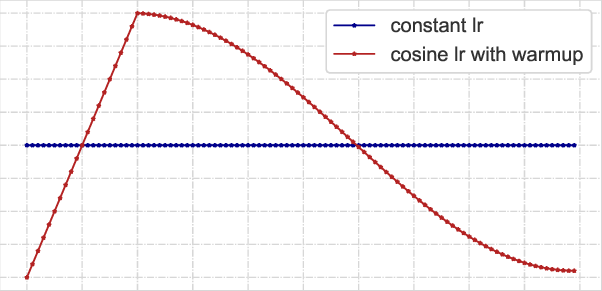
\includegraphics[width=0.7\textwidth]{cosine-annealing-lr-with-warmup.png}
    \caption[Cosine annealing LR]{\label{fig:cosine_annealing_lr}. Vergelijking tussen constante \gls{learning_rate} en \gls{learning_rate} aangepast door een Cosine Annealing LR-scheduler met warm-up. \autocite{Lu_2019}}
\end{figure}

Dit geoptimaliseerd model werd echter niet gebruikt in het uiteindelijke onderzoek om de resultaten zo goed mogelijk met de originele paper van \textcite{Xie_2022} te kunnen vergelijken enerzijds en omdat de performantie van het model ondermaats was anderzijds.

% Semi-supervised model (FixMatch)
\section{Semi-supervised learning: principes en technieken}

\subsection{Definitie en waarde binnen objectdetectie}

Binnen het domein van machine learning bestaan er verschillende technieken om een model te trainen. Meestal wordt er gesproken van twee grote stromingen: supervised learning en unsupervised learning. Bij supervised learning wordt er gebruik gemaakt van een dataset en een uitkomst (hetgeen het model uiteindelijk moet kunnen voorspellen). Dit kan een label zijn of een bepaalde numerieke waarde. Belangrijk is dat zowel de input als de gewenste output gegeven zijn. Het model leert dus het verband tussen de twee. Bij unsupervised learning zijn er geen verwachte outputs. De volledige dataset wordt door het model gebruikt om patronen in te herkennen. Unsupervised learning wordt daarom ook meestal gebruikt om verkennende data-analyse uit te voeren. Echter hebben beide methoden enkele nadelen. Bij supervised learning is het traag en duur om alle data op een correcte manier te labelen. Unsupervised learning heeft dit probleem niet, maar heeft een beperkt aantal toepassingen en is minder accuraat. Een alternatief is \gls{ssl}, wat een compromis tussen zowel supervised als unsupervised learning is. \autocite{C_A_Padmanabha_Reddy_2018} \\

\gls{ssl} is een subdomein van machine learning waar gebruik gemaakt wordt van zowel gelabelde als ongelabelde data om modellen te trainen. Dit is bijzonder nuttig in situaties waarin het labelen van gegevens duur of tijdrovend is, zoals bij sonardata het geval is. \gls{ssl} bevindt zich tussen supervised learning (waar alle trainingsdata gelabeld zijn) en unsupervised learning (waar geen labels beschikbaar zijn). Door gebruik te maken van een kleine hoeveelheid gelabelde gegevens in combinatie met een grote hoeveelheid ongelabelde gegevens, kan een model beter generaliseren waardoor de prestaties verbeteren met minder menselijke annotatie-inspanning. \autocite{Hady_2013} \\

Zoals eerder vermeld, is \gls{ssl} een subdomein van machine learning, net zoals supervised en unsupervised learning. Het is dus niet één model of één architectuur, maar een waaier van verschillende algoritmen die soms op hele andere manieren werken. Wel hebben ze allemaal gemeen dat ze zowel gelabelde als ongelabelde data gebruiken. \\

Één van de belangrijkste technieken binnen \gls{ssl} is \emph{consistency regularization} (cf. infra), waarbij een model wordt aangemoedigd om consistente voorspellingen te maken voor kleine verstoringen van dezelfde ongelabelde input. \autocite{Fan_2022} Een ander veelgebruikt principe is \emph{pseudo-labeling} (cf. infra), waarbij het model zelf voorspellingen genereert voor ongelabelde gegevens en deze gebruikt als extra trainingsdata. \autocite{Lee_2013} \\

Daarnaast is er graph-based \gls{ssl}. Dit is een techniek die gebruik maakt van grafen (netwerken) om de relaties tussen gelabelde en ongelabelde data te modelleren en labelinformatie effectiever te verspreiden. In plaats van uitsluitend te vertrouwen op individuele gegevenspunten, gebruiken deze methoden de structuur van de dataset om aannames te maken over onbekende labels. Dit is vooral nuttig in situaties waarin de onderliggende data een natuurlijke connectiviteit vertoont, zoals sociale netwerken, biologische netwerken en tekstanalyses. \autocite{Song_2021} \\

Graph-based \gls{ssl}-modellen stellen de dataset voor als een graaf $G = (V, E)$ waarbij $V$ de knopen (datapunten) zijn (zowel gelabelde als ongelabelde gegevens) en $E$ de de gewogen randen (connecties) tussen knopen zijn, die de relatie of gelijkenis tussen de datapunten aangeven. Het basisidee is dat naburige knopen waarschijnlijk tot dezelfde klasse behoren, een principe dat bekend staat als \emph{label propagation}. Labels van bekende knopen (gelabelde data) worden hierbij iteratief verspreid naar naburige knopen op basis van de sterkte van de verbindingen. \autocite{Zhu_2005} \\

\gls{ssl} wordt toegepast in diverse domeinen, zoals beeld- en spraakherkenning, biomedische analyse en autonome systemen. Recente ontwikkelingen in deep learning hebben geleid tot geavanceerde \gls{ssl}-methoden, zoals FixMatch en MixMatch (cf. infra), die de prestaties aanzienlijk verbeteren door sterke data-augmentatie, efficiënter gebruik van ongelabelde data en de combinatie van andere \gls{ssl}-technieken. Onderzoek heeft aangetoond dat \gls{ssl} met slechts 10\% gelabelde data al bijna dezelfde prestaties kan bereiken als volledig gelabelde modellen. \autocite{Lucas_2022}

\subsection{Veelgebruikte SSL-methoden}

\acrfull{ssl} omvat verschillende methoden die gebruik maken van zowel gelabelde als ongelabelde data om de prestaties van machine learning-modellen te verbeteren. Veelgebruikte \gls{ssl}-methoden compenseren de beperkte beschikbaarheid van gelabelde data door patronen en structuren in ongelabelde data te benutten. \gls{ssl} wordt voor alle soorten doeleinden gebruikt: niet alleen in predictieve modellen, waarbij er vaak gebruik gemaakt wordt van pseudo-labeling en consistency regularization, wordt \gls{ssl} ingezet. Ook bij generatieve modellen wordt \gls{ssl} enorm veel gebruikt. Dit gaat dan bijvoorbeeld om \glspl{vae} en \glspl{gan}. Deze worden hierbij ingezet om aanvullende trainingsgegevens te genereren. Door al deze technieken te combineren, kunnen \gls{ssl}-methoden significante verbeteringen bieden voor taken zoals beeldherkenning, spraakverwerking en \gls{nlp}. \autocite{van_Engelen_2019} Hieronder worden enkele van de meest prominente technieken binnen \gls{ssl} besproken.

\subsubsection{Pseudo-labeling}

Pseudo-labeling is een belangrijke techniek binnen \gls{ssl} waarbij een model, getraind op een beperkte hoeveelheid gelabelde data, wordt ingezet om voorspellingen te doen op ongelabelde data. Deze voorspellingen, aangeduid als ``pseudo-labels'', worden vervolgens behandeld als echte labels, waardoor het model verder kan worden verfijnd met een uitgebreidere dataset. Dit proces wordt iteratief herhaald, zodat het model geleidelijk aan zijn prestaties verbetert door zowel de gelabelde als de pseudo-gelabelde data te gebruiken. \autocite{Lee_2013} \\

Het succes van pseudo-labeling is natuurlijk afhankelijk van de nauwkeurigheid van de gegenereerde pseudo-labels. Om de kwaliteit te waarborgen, wordt vaak een drempelwaarde ingesteld voor de voorspellingszekerheid: alleen voorspellingen die boven deze drempel uitkomen, worden als pseudo-labels geaccepteerd. Dit helpt het model om zich te concentreren op voorbeelden waarbij het relatief zeker is van de voorspelling, waardoor het risico op het leren van verkeerde informatie wordt verminderd. \autocite{Kage_2024} \\

Een belangrijk voordeel van pseudo-labeling is dat het effectief gebruikmaakt van grote hoeveelheden ongelabelde data, wat vooral nuttig is in domeinen zoals sonarbeeldvorming, waar het verkrijgen van gelabelde data duur en tijdrovend is. Verder zijn toepassingen van pseudo-labeling te vinden in verschillende gebieden, waaronder beeldherkenning, spraakverwerking en \gls{nlp}. \autocite{Min_2022} Recent onderzoek van \textcite{Ferreira_2023} heeft aangetoond dat pseudo-labeling een zeer goede performantie kan neerzetten, terwijl het de behoefte aan uitgebreide gelabelde datasets vermindert. \\

Desondanks kent pseudo-labeling ook uitdagingen. Als het model in een vroeg stadium onnauwkeurige pseudo-labels genereert, kan dit leiden tot het versterken van fouten, een fenomeen bekend als \emph{confirmation bias}. Om dit te voorkomen, worden technieken zoals \emph{curriculum learning} toegepast, waarbij het model eerst wordt getraind met de meest zekere pseudo-labels en geleidelijk aan minder zekere voorbeelden toevoegt naarmate de training vordert. \autocite{Cascante_Bonilla_2020}

\subsubsection{Consistency Regularization}

Een ander fundamenteel concept binnen \gls{ssl} is consistency regularization. Deze techniek wordt in verschillende algoritmen gebruikt om de betrouwbaarheid van het model te verbeteren. Het doet dit door het model te dwingen consistente voorspellingen te maken voor kleine variaties van dezelfde input. Het idee is gebaseerd op de veronderstelling dat een model robuust moet zijn tegen kleine verstoringen in de input, vooral wanneer de input geen gelabelde gegevens bevat. \\

Eerst wordt een ongelabeld voorbeeld $x_u$ aangepast met kleine verstoringen. Dit kan gaan om data-augmentatie (bv. willekeurige rotaties, verscherping, kleuraanpassingen, \dots), het toevoegen van ruis (bv. Gaussian noise), \dots Dit resulteert in twee versies van dezelfde input: het origineel $x_u$ en de verstoorde versie $x'_u$. Daarna voorspelt het model de kansverdeling van de klassen voor zowel de originele als de verstoorde input. \\

Een consistente voorspelling betekent dat beide kansverdelingen ``dicht'' bij elkaar moeten liggen. Om dit te garanderen wordt een gespecialiseerde \gls{loss_functie} gebruikt, zoals de \gls{kl}-divergentie \autocite{Hall_1987} of de \gls{mse}. Het model wordt getraind om deze \emph{loss} te minimaliseren, zodat het stabiele en robuuste voorspellingen leert maken, zelfs bij verstoringen. \\

Consistency regularization is enorm effectief (en wordt daarom ook veel gebruikt) omdat het ervoor zorgt dat het model gebruik maakt van de onderliggende structuur van ongelabelde data. Hierdoor verbetert de generalisatie, omdat het model minder gevoelig wordt voor kleine ruis en variaties. Daarnaast verhoogt de sample-efficiëntie, waardoor minder gelabelde data nodig is voor goede prestaties. \autocite{Fan_2022}

\subsubsection{MixMatch en FixMatch}

\lipsum[1]

% Self-supervised model (BYOL)
\section{Self-supervised learning: principes en technieken}

\subsection{Definitie en verschil met SSL}

Anders dan bij \gls{ssl} is er bij \gls{self-sl} helemaal geen nood aan labels. Deze creëert het algoritme namelijk zelf tijdens een pre-training fase. Semi-supervised learning behoort echter niet helemaal tot het domein van unsupervised learning, hoewel het gebruik maakt van verschillende groeperings- en clusteringmethoden. Het uiteindelijke model maakt namelijk gebruik van -- door de pre-training -- gelabelde data. Deze techniek zorgt ervoor dat er veel complexere modellen getraind kunnen worden zonder een gigantische hoeveelheid aan data. Enkele nadelen zijn wel dat de techniek een grote hoeveelheid computerkracht nodig heeft en een lagere accuratie heeft dan supervised learning. \autocite{Gui_2024} \\

Het fundamentele verschil tussen self-supervised en semi-supervised learning ligt in de manier waarop ze omgaan met labels. In semi-supervised learning zijn er externe, door mensen geannoteerde labels aanwezig, zij het in beperkte mate. Self-supervised learning genereert daarentegen volledig zijn eigen labels zonder externe annotaties. Hierdoor wordt self-supervised learning soms beschouwd als een vorm van unsupervised learning, maar met expliciet gedefinieerde pretext-taken om de onderliggende structuren in data beter te benutten. \\

Ondanks deze nadelen blijken verschillende populaire technieken succesvol binnen het domein van computer vision.

\subsection{Werking}

\autocite{Oord_2018}

\lipsum[1]

\subsection{Veelgebruikte Self-SL methoden}

In de context van vooruitgang in \gls{ssl} zijn er verschillende praktische modellen ontwikkeld die de eerder besproken theoretische principes -- zoals contrastive learning en representatieleren zonder gelabelde data -- succesvol toepassen op grootschalige visuele data. Deze modellen onderscheiden zich niet alleen door hun architecturale keuzes, maar ook door hoe ze omgaan met negatieve samples, augmentatiestrategieën en het gebruik van momentum-updates. In deze sectie worden enkele invloedrijke en veelgebruikte \gls{ssl}-methoden besproken in realistische settings, met een focus op \acrfull{simclr}, \acrfull{moco} en \acrfull{byol}. Elk van deze modellen illustreert op unieke wijze hoe self-supervised representaties kunnen worden geleerd met minimale supervisie, en vormt daarmee een belangrijke bouwsteen in moderne computer vision toepassingen.

\subsubsection{SimCLR}

Een bekende \gls{self-sl}-techniek is \acrshort{simclr}. Deze afkorting staat voor \acrlong{simclr}. Met andere woorden maakt deze techniek dus gebruik van \emph{contrastive learning} om visuele representaties te leren zonder de noodzaak van gelabelde data. Het werd ontwikkeld door onderzoekers van Google Brain en gepresenteerd in een paper van \textcite{Chen_2020}. Het doel van \gls{simclr} is om een neuraal netwerk zodanig te trainen dat het visuele representaties van afbeeldingen leert door contrastieve relaties te benutten.

Om een model contrastieve representaties te laten leren, worden er van elke invoerafbeelding eerst twee willekeurige transformaties gemaakt. Deze transformaties kunnen bestaan uit verschillende dingen, waaronder:

\begin{itemize}
    \item Willekeurig bijsnijden en schalen
    \item Kleurveranderingen zoals de helderheid en contrast aanpassen
    \item Toepassen van blurring
    \item Rotatie of horizontale spiegeling
\end{itemize}

Deze transformaties zorgen ervoor dat het model leert om dezelfde afbeelding te herkennen, ongeacht variaties in uiterlijk. Na de augmentaties worden de twee versies van de afbeelding door een encoder gestuurd, meestal een \gls{cnn} (zoals een ResNet). Dit netwerk zet de invoerafbeeldingen om in zogenaamde \emph{feature vectors} die de kernkenmerken van de afbeelding representeren. \\

De gegenereerde feature vectors worden vervolgens door een \emph{projection head} gestuurd. Dit is een klein neuraal netwerk dat de feature vector transformeert naar een ruimte waarin de contrastieve vergelijking plaatsvindt (latente ruimte). Dit projection head bestaat meestal uit een paar  fully connected of dense-lagen en wordt na training weggegooid, omdat alleen de encoder nodig is voor downstream taken (zoals beeldclassificatie, objectdetectie en semantische segmentatie). \autocite{Gupta_2022} \\

Het doel van SimCLR is om representaties van verschillende augmentaties van dezelfde afbeelding dichter bij elkaar te brengen en representaties van verschillende afbeeldingen verder uit elkaar te duwen. Dit gebeurt met behulp van de \gls{nt-xent} loss. De \gls{loss_functie} wordt berekend zodat positieve paren (twee augmentaties van dezelfde afbeelding) een hoge gelijkenis hebben en negatieve paren (verschillende afbeeldingen in de \gls{batch}) een lage gelijkenis. De cosinusgelijkheid wordt vaak gebruikt om de afstand tussen de verschillende vectoren te meten. Daarnaast beïnvloedt de temperatuurparameter $\tau$ in de \gls{nt-xent} loss  hoe streng de loss reageert op verschillen in gelijkenis tussen paren.

\subsubsection{MoCo}

Een andere veelgebruikte \gls{self-sl}-techniek is \gls{moco}. Deze methode maakt gebruik van contrastief leren om visuele representaties te leren zonder de noodzaak van gelabelde data. Het werd geïntroduceerd in een paper van \textcite{He_2019} en heeft sindsdien aanzienlijke aandacht gekregen binnen het domein van de computer vision. \gls{moco} introduceert verschillende innovatieve technieken zoals het \emph{momentum update}-mechanisme en een dynamisch woordenboek om contrastief leren te verbeteren. Ook wordt er een gespecialiseerde \gls{loss_functie} gebruikt die de basis vormt van het leerproces. Dankzij deze strategieën kan \gls{moco} superieure representaties leren zonder gelabelde data, wat het een krachtige \gls{self-sl}-techniek maakt. \\

Het \gls{moco}-framework bestaat uit meerdere essentiële componenten die samenwerken om effectieve visuele representaties te leren. De \emph{query encoder} ($f_q$) is verantwoordelijk voor het omzetten van een \emph{query sample} (zoals een geaugmenteerde versie van een afbeelding) in een \emph{feature vector}. De parameters van deze encoder worden bijgewerkt via standaard backpropagation, waarbij de optimalisatie wordt gestuurd door een contrastieve \gls{loss_functie}. \autocite{Sowe_2025} \\

Daarnaast bevat \gls{moco} een \emph{momentum key encoder} ($f_k$) die wordt gebruikt om \emph{keys} (bijvoorbeeld geaugmenteerde weergaven uit eerdere \glspl{mini_batch}) om te zetten in \emph{feature vectors}. Een cruciale innovatie van \gls{moco} is het \emph{momentum update}-mechanisme. In plaats van direct via backpropagation te worden bijgewerkt, worden de parameters van de \emph{key encoder} ($\theta_k$) aangepast als een voortschrijdend gemiddelde van de \emph{query encoder} ($\theta_q$). Dit gebeurt volgens de volgende formule:

$$
\theta_k \rightarrow m\theta_k + (1 - m)\theta_q
$$

Hierbij is $m$ de \emph{momentumcoëfficiënt}, die doorgaans dicht bij 1 ligt (bv. 0,999). Dit zorgt voor een geleidelijke en stabiele update van de key encoder, waardoor de representaties van de keys na verloop van tijd minder variëren. Een stabieler woordenboek van negatieve samples is cruciaal voor contrastief leren, omdat het helpt om robuuste en onderscheidende kenmerken te leren. \\

Om een grote en gevarieerde set van negatieve samples te behouden, maakt \gls{moco} gebruik van een dynamisch woordenboek dat wordt beheerd via een FIFO (First-In, First-Out) wachtrij. Dit mechanisme zorgt ervoor dat de grootte van het woordenboek niet wordt beperkt door de mini-batchgrootte, zoals bij traditionele contrastieve leermethoden het geval is.

\begin{itemize}
    \item Wanneer een nieuwe mini-batch wordt verwerkt, worden de bijbehorende representaties aan het einde van de wachtrij toegevoegd (enqueue).
    \item Tegelijkertijd worden de oudste representaties uit de wachtrij verwijderd (dequeue).
\end{itemize}

Dit ontkoppelt het aantal negatieve samples van de batchgrootte, waardoor \gls{moco} kan werken met veel grotere negatieve sets zonder dat dit een grote hoeveelheid GPU-geheugen vereist. Een groter en gevarieerder aantal negatieve samples helpt het model om betere representaties te leren, omdat de contrastieve taak uitdagender wordt. Dit dwingt het model om robuustere en meer onderscheidende kenmerken te ontwikkelen. \\

\gls{moco} maakt gebruik van de InfoNCE loss, een contrastieve verliesfunctie die het model leert om:

\begin{enumerate}
    \item De gelijkenis tussen een query en zijn bijbehorende positieve key te maximaliseren (dit zijn verschillende augmentaties van dezelfde afbeelding).
    \item De gelijkenis tussen de query en negatieve keys te minimaliseren (deze representeren andere afbeeldingen in de wachtrij).
\end{enumerate}

De wiskundige formulering van de InfoNCE loss is als volgt:

$$
L_q = - \log \frac{\exp{(q \cdot k^+ / {\tau})}}{\sum_{i=0}^{K}\exp{(q \cdot k_i / {\tau})}}
$$

Hierbij geldt:

\begin{itemize}
    \item $q =$ de gecodeerde query
    \item $k^+ =$ de gecodeerde positieve key
    \item $k_i =$ alle keys in het woordenboek (inclusief $k^+$ en $K$ negatieve keys)
    \item $\tau =$ de temperatuurparameter, die de scherpte van de loss controleert  
\end{itemize}

De InfoNCE loss vormt de kern van het leerproces van \gls{moco} en stelt het model in staat om een embedding space te creëren waarin augmentaties van dezelfde afbeelding dicht bij elkaar liggen en representaties van verschillende afbeeldingen ver uit elkaar worden geplaatst. Dit proces, bekend als \emph{instance discrimination}, helpt het model om semantisch betekenisvolle kenmerken te leren zonder gelabelde data.

\subsubsection{BYOL}

%\autocite{Adaloglou_2022}

Naast de contrastieve methoden die veelal gebruikt worden binnen het domein van \gls{self-sl} is er sinds enkele jaren ook een ander alternatief. \gls{byol} is ontwikkeld bij Google DeepMind en werd geïntroduceerd in een paper van \textcite{Grill_2020}. \gls{byol} is gebaseerd op het idee dat een model kan leren door zijn eigen representaties te gebruiken als leersignaal. Dit gebeurt door twee verschillende, geaugmenteerde versies van hetzelfde inputbeeld te genereren, en het model leert vervolgens om de representatie van de ene versie te voorspellen op basis van de andere. In tegenstelling tot contrastieve leermethoden -- die gebruikmaken van zowel positieve als negatieve paren -- werkt \gls{byol} volledig zonder negatieve voorbeelden. Terwijl contrastieve methoden proberen representaties van verschillende beelden uit elkaar te duwen, focust \gls{byol} zich enkel op het dichter bij elkaar brengen van representaties van dezelfde onderliggende input. Deze aanpak vermindert de kans op instabiliteit en maakt het model robuuster voor variaties in data-augmentatie. \\

Het leerproces in \gls{byol} is gebouwd op twee samenwerkende netwerken: een \emph{online netwerk} en een \emph{target netwerk}. Het online netwerk probeert de representatie te voorspellen die door het target netwerk is gegenereerd. Het target netwerk zelf wordt niet direct getraind via \gls{backpropagation}, maar geüpdatet via een \gls{ema} van de parameters van het online netwerk. Deze samenwerking tussen de twee netwerken zorgt voor een geleidelijke en stabiele leeromgeving. \\

Zoals hierboven vermeld, bestaat de \gls{byol}-architectuur dus twee identieke netwerken qua structuur: het online netwerk en het target netwerk. Het online netwerk bevat drie componenten:

\begin{enumerate}
    \item \textbf{Encoder ($f_\theta$):} extraheert een representatie uit een geaugmenteerd inputbeeld.
    \item \textbf{Projector ($g_\theta$):} projecteert deze representatie naar een lagere-dimensionale vectorruimte.
    \item \textbf{Predictor ($q_\theta$):} probeert de representatie van het target netwerk te voorspellen.
\end{enumerate}

Het target netwerk bevat alleen de encoder en projector, zonder predictor. Het wordt bijgehouden als een langzame, voortschrijdende kopie van het online netwerk, waardoor het stabielere leerdoelen biedt. Tijdens training worden twee verschillende augmentaties van eenzelfde afbeelding verwerkt: één door het online netwerk en de andere door het target netwerk. Het doel is dat de output van de predictor van het online netwerk overeenkomt met de projectie van het target netwerk. \\

De \gls{loss_functie} voor \gls{byol} is gebaseerd op de \gls{mse} tussen L2-genormaliseerde vectoren: de voorspelling van het online netwerk en de projectie van het target netwerk. \autocite{Laarhoven_2017} Voor een enkel augmentatiepaar $(v, v')$ wordt de loss als volgt berekend:

$$
L_{\theta, \xi} = \left\Vert \text{normalize}\left(q_\theta\left(z_\theta\right)\right) - \text{normalize}\left(z'_\xi\right) \right\Vert^2_2 = 2 - 2 \cdot \left\langle \text{normalize}\left(q_\theta\left(z_\theta\right)\right), \text{normalize}\left(z'_\xi\right) \right\rangle
$$

Data-augmentatie speelt een centrale rol in \gls{byol}. Door willekeurige transformaties toe te passen (zoals crops, kleurvervormingen, flips, \dots), ontstaan twee verschillende maar inhoudelijk gelijke views van hetzelfde beeld. Deze variatie dwingt het model om representaties te leren die geen rekening houden met oppervlakkige veranderingen en gericht zijn op de semantische kern van het beeld. Interessant is dat \gls{byol} minder gevoelig is voor de specifieke keuze van augmentaties dan contrastieve methoden zoals \gls{simclr}. Het model blijft effectief presteren, zelfs wanneer bepaalde augmentaties worden weggelaten, wat wijst op een grotere robuustheid.